\begin{frame}{Ein Angebot}
  \centering
  
  \note<1->[item]{Nachgrübeln was zu tun}
  \note<1->[item]{Plötzlich ein Angebot}
  \note<2->[item]{Firma "Data Broker GmbH" will Firma übernehmen \begin{itemize}
      \item Bietet Geld. (KLICK) VIEL Geld
  \end{itemize}}
  \note<4->[item]{Mitarbeiter fragen sich: Woher der hohe Preis?}
  \note<4->[item]{Gesammelte Daten sind nur für Transaktionen Wichtige}
  
  \begin{tikzpicture}
    \node<1-3> (walter) {
\includegraphics[width=0.15\textwidth]{images/walter.png}};
    \node<1-3>[below=0mm of walter] (walter-name) {Walter};
    
    \node<2-3>[right=4cm of walter] (databroker) {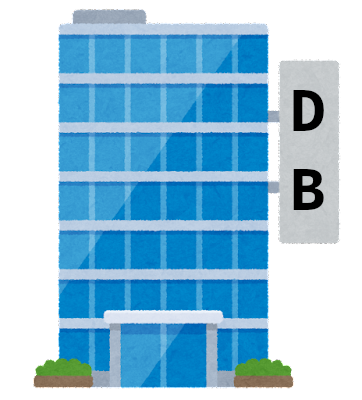
\includegraphics[width=0.15\textwidth]{images/data_broker.png}};
    \node<2-3>[below=0cm of databroker] (databroker-name) {Data Broker GmbH};
    
    % Data Broker kommt
    
    \draw<2-3>[stealth-] ([yshift=1mm]databroker.west) -- node[above] (acgames-name) {AC-Games}  ([yshift=1mm]walter.east);
    \node<2-3>[above=0cm of acgames-name] (acgames) {
\includegraphics[width=0.075\textwidth]{images/ac_games.png}};
    \draw<2>[stealth-] ([yshift=-1mm]walter.east) -- node[below] {
\includegraphics[width=0.075\textwidth]{images/dollar_bill.png}}  ([yshift=-1mm]databroker.west);
    
    % MORE MONEY
    
    \draw<3>[stealth-] ([yshift=-1mm]walter.east) -- node[below] {
\includegraphics[width=0.1\textwidth]{images/money_bag_dollar.png}} ([yshift=-1mm]databroker.west);
    
    % Warum so viel geld?
    
    \node<4-> (typ) {
\includegraphics[width=0.45\textwidth]{images/pose_shinpai_fukidashi_man.png}};
    \node<4->[above=0cm of typ.center] (money) {
\includegraphics[width=0.18\textwidth]{images/money_bag_dollar.png}};
    
  \end{tikzpicture} 
\end{frame}

\begin{frame}{Ein Angebot}
  \centering
  
  \note[item] {Pro \begin{itemize}
      \item Firma bleibt relativ sicher bestehen
      \item Spieler und ihr Investment werden nicht im Stich gelassen
  \end{itemize}}
  \note[item]{Contra \begin{itemize}
      \item Daten in der Hand von Datenhändler \begin{itemize}
          \item Hoher Preis wird wohl seinen Grund haben
          \item Wahrscheinlich nicht aus reiner Wohltat
      \end{itemize}
  \end{itemize}}
  \note[item]{Alternativen \begin{itemize}
      \item Crowdfunding
      \item Vielleicht an dieser Stelle zu spät, aber hätte sich ein anderes Produkt überlegen können \begin{itemize}
          \item Haben ja schon Jahre vorher gemerkt, dass es mit ihrem Produkt abwärtsgeht
      \end{itemize}
  \end{itemize}}
  
  \Large
  Sollte Walter AC-Games an Data Broker verkaufen?\\
  Wenn nein, gibt es eine Alternative?
  
  
\includegraphics[width=0.425\textwidth]{images/discussion.png}
\end{frame}

\begin{frame}{Ein Angebot}
  \centering
  
  \note[item] {Pro \begin{itemize}
    \item Offensichtlich: Firma soll überleben
  \end{itemize}}
  \note[item]{Contra \begin{itemize}
    \item Finanzkrise ist ja nicht einziger Grund
    \item App Stores etc. bieten scheinbar besseren Service
    \item In-Game Käufe lassen nach $\Rightarrow$ hört sich eher nach Problem mit Produkt selbst an
  \end{itemize}}
  
  \Large
  Wie bewertet ihr, dass AC-Games trotz finanzieller Schwierigkeiten ihr Portal weiter betreiben wollen? 
  
  
\includegraphics[width=0.425\textwidth]{images/discussion.png}
\end{frame}
